\documentclass[12pt]{article}
\usepackage{amsmath}
\usepackage{amssymb}
\usepackage{geometry}
\usepackage{enumerate}
\usepackage{natbib}
\usepackage{float}%稳定图片位置
\usepackage{graphicx}%画图
\usepackage[english]{babel}
\usepackage{a4wide}
\usepackage{indentfirst}%缩进
\usepackage{enumerate}%加序号
\usepackage{multirow}%合并行
\title{\large UM-SJTU JOINT INSTITUTE\\PHYSICS LABORATORY\\(VP241)\\\ \\\ \\\ \\\ \\\ \\\ \\\ \\\ \\\ \\\ \\\
LABORATORY REPORT\\\ \\\ EXERCISE 3\\\ Solar Cells: I-V Characteristics \\\ \\\ \\\ \\\ \\\ }
\author{Name: Pan Chongdan \\ID: 516370910121\\Partner:Chen Yuxin\\ID:516370910128\\Group: 6}
\date{Date: \today}

\begin{document}
\maketitle
\newpage
\section{Objectives}
\begin{enumerate}
\item To get familiar with the working principle of a solar cell.
\item Study the solar cell's current-voltage characteristics.
\end{enumerate}
\section{Introduction and Theoretical Background}
Solar cells can transform solar radiation into electrical energy directly. They're very useful because they won't consume energy and it's operation is silent. It also has a long lifetime without moving parts. In addition, they are easy to maintain and never cause air pollution. Therefore, they become one of the leading energy sources because they can produce 15-20$\%$ of the total electrical energy generated in the world. 
\subsection{Solar Cell Structure}
A crystalline silicon solar cell consists of $\frac{n}{p}$ homo-junctions, a 10 cm
$\times$ 10 cm $p-$type silicon plate of thickness 500 $\mu m$, covered with a heavily doped $n-$type layer with thickness 0.3 $\mu m$. The metallic balls on the $n-$ type layer is like an electrode with a metallic film at the bottom playing the role of another one. To reduce the loss of energy caused by reflection, an anti-reflective film is often used to cover the surface exposed to light.
\begin{figure}[H]
\centering
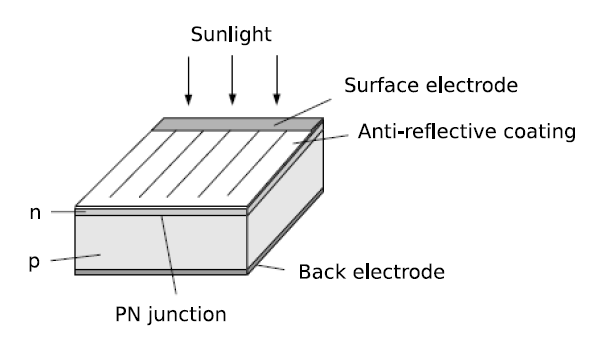
\includegraphics[scale=0.5]{P1.jpg}
\caption{Structure of a crystalline silicon solar cell.}
\end{figure}
\subsection{Photovoltaic Effect}
The incident photons are absorbed and excite electron pairs when the light enters the p-n junction near the solar cell surface, and the energy of incident photons is greater than the forbidden bandwidth $E_g$.Minority charge carriers in the n- or
p-type area diffuse due to their density gradient. Some of them are able to diffuse to the
region of the p-n junction where a built-in electric field exists, which is directed from
the n-type to the p-type area. The minority carriers diffusing to the p-n junction zone
between the n-type area and the p-type area are drawn by this electric field to the p-type
area, or to the n-type area. This cause more positive charge accumulated in the p-type area and negative charge in the n-type area. Therefore, a photoelectric potential difference is generated.
\subsection{Solar Cell Parameters}
Solar cells can generate an electric current $I_{ph}$ from the $n$-type area to the $p$-type area when there is light incident on the solar cell due to the photovoltaic effect.
\par At the same time, a forward diode current $I_D$ from  the $p$-type to the $n$-type area  exists in the device, which has an opposite direction to $I_{ph}$. As a result, the net current:
\begin{equation}
I=I_{ph}-I_D=I_{ph}-I_0[\mathrm{exp}(\frac{dV_D}{nk_BT})-1]
\end{equation}	
where $V_D$ is the junction voltage, $I_0$ is the diode inverse saturation current, $I_{ph}$ is the photo current determined by the structure and material characteristics of the solar cell. The coefficient $n$ is a theoretical coefficient whose value ranges from 1 to 2, which characterizes the $p-n$ junction. Additionally, $q,k_B,T$ denote the electron's charge, Boltzmann's constant, and temperature in the Kelvin scale respectively. If we ignore the internal resistance $R_S$, $V_D$ will equals to the terminal voltage $V$ ,so 
$$I=I_{ph}-I_0[\mathrm{exp}(\frac{dV}{nk_BT})-1]$$
\begin{enumerate}
\item If the output circuit is short so $V=0$, then 
$$I_{sc}=I_{ph}$$
\item If the output circuit is open so $I=0$, then
$$V_{oc}=\frac{nk_BT}{q}\ln(\frac{I_{sc}}{I_0}+1)$$
\item If there is a load resistance $R$, the corresponding $I-V$ characteristic curve is shown in Figure 2. When the maximum power $P_m$ is generated with $R=R_m,I=I_m,V=V_m$, then 
$$FF=\frac{P_m}{V_{oc}I_{sc}}=\frac{V_mI_m}{V_{oc}I_{sc}}$$
\begin{figure}[H]
\centering
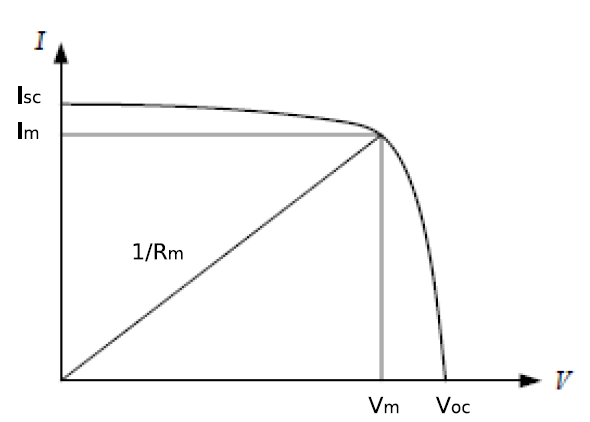
\includegraphics[scale=0.7]{P2.jpg}
\caption{The current-voltage characteristics of a solar cell.}
\end{figure}
\end{enumerate}
$FF$ is called the $fill factor$, which is very important and it's determined by some parameters such as the incident light intensity, the forbidden bandwidth, the value of
the theoretical coefficient $n$, and the series/parallel resistance.
\par The solar cell energy conversion efficiency $\eta$ is defined as
$$\eta=\frac{P_m}{P_{in}}\cdot 100\%$$
where $P_{in}$ denotes the total radiant power incident on the solar cell.
\subsection{Solar Cell Equivalent Circuit}
\begin{figure}[H]
\centering
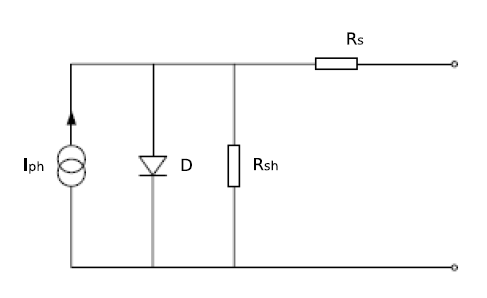
\includegraphics[scale=0.5]{P3.jpg}
\caption{Solar cell equivalent circuit.}
\end{figure}
The figure 3 shows that a solar cell can be thought of as composed of $p-n$ junction diode $D$ and a constant current source $I_{ph}$ along with a series resistance $R_s$ due to
the electrodes in the solar cell and a parallel resistance $R_{sh}$, all elements form a circuit equivalent to a $p-n$ junction leak-circuit. The relation between the current and the voltage,
$$I=I_{ph}-I_0\{\mathrm{exp}[\frac{q(V+R_sI)}{nk_BT}]-1\}-\frac{V+R_SI}{R_{sh}}$$
We can decrease $R_s$ and increase $R_{sh}$ to provide a greater power.
\section{Measurement Set up and Procedure}
\subsection{Measurement Set up}
The set up consists of a 5W photovoltaic device, a 300W tungsten-halogen lamp serving as a radiation source, two digital multimeter, two adjustable resistors, a solar power meter, a wiring board and a measuring tape.
\subsection{Measurement Procedure and Data Presentation}
\begin{enumerate}
\item I turned on the light and the fan, then waited for a few minutes until the light reach its working intensity.
\item I designed a measuring circuit with the photovoltaic device, multimeter sets in an appropriate range, and the resistance and connected the elements into a circuit using the provided wiring board.
\item I changed resistance and measured the relevant current and voltage to draw the $I-V$ characteristic curve.
\item I measured the $I-V$ characteristic curves and the values of $V_{oc}$ and $I_{sc}$ under four conditions:
\begin{enumerate}[i]
\item The distance between the light source and the photovoltaic device is 100 cm.
\item The distance between the light source and the photovoltaic device is 120 cm.
\item The distance between the light source and the photovoltaic device is 120 cm,
with two devices in series.
\item The distance between the light source and the photovoltaic device is 120 cm,
with two devices in parallel.
\end{enumerate}
\item I plot the $I-V$ characteristic curves and the graph of the output power to determine the values of $I_{sc},V_{oc},P_m,I_m,V_m,R_m,FF$ and $\eta$.
\end{enumerate}  
\section{Results and Calculation}
\subsection{Measurement Data}
\begin{table}[H]
\centering
\begin{tabular}{|c|c|}
\hline
Quantity    & Precision \\ \hline
DC voltage  & $0.5\%\pm0.01$[V]       \\ \hline
DC current  & $1.5\%\pm0.1$[mA]   
    \\ \hline
distance    & 0.1[cm]       \\ \hline
solar power & 10[W/m$^2$]        \\ \hline
\end{tabular}
\caption{Multimeter precision}
\end{table}
\begin{table}[H]
\centering
\begin{tabular}{|c|c|}
\hline
Length[cm] & Width[cm] \\ \hline
20.9       & 26.2      \\ \hline
\end{tabular}
\caption{Measurement data for area}
\end{table}
\begin{table}[H]
\centering
\begin{tabular}{|c|c|c|c|c|c|}
\hline
 & 0   & 1   & 2   & 3   & 4   \\ \hline
$P_{100}$[W/m$^2$] & 213 & 265 & 240 & 237 & 295 \\ \hline
$P_{120}$[W/m$^2$] & 206 & 240 & 182 & 163 & 255 \\ \hline
\end{tabular}
\caption{Measurement data for solar power}
\end{table}
\begin{table}[H]
\centering
\begin{tabular}{|c|c|c|c|c|}
\hline
 & 100cm & 120cm & series & parallel \\ \hline
$U_{oc}$[V] & 8.91  & 8.38  & 18.06  & 9.01     \\ \hline
$I_{sc}$[mA] & 83.2  & 72.4  & 77.2   & 146.7    \\ \hline
\end{tabular}
\caption{Measurement data for $U_{oc}$ and $I_{sc}$}
\end{table}
\begin{table}[H]
\centering
\begin{tabular}{|c|c|c|c|c|}
\hline
   & \multicolumn{2}{c|}{100cm} & \multicolumn{2}{c|}{120cm} \\ \hline
   & U[V]        & I[mA]        & U[V]        & I[mA]        \\ \hline
1  & 0.44        & 83.0         & 0.39        & 73.7         \\ \hline
2  & 0.78        & 82.1         & 0.72        & 72.9         \\ \hline
3  & 1.12        & 81.6         & 1.05        & 72.2         \\ \hline
4  & 1.46        & 80.8         & 1.38        & 71.5         \\ \hline
5  & 1.80        & 80.0         & 1.71        & 70.5         \\ \hline
6  & 2.14        & 78.8         & 2.04        & 69.4         \\ \hline
7  & 2.48        & 77.8         & 2.37        & 68.6         \\ \hline
8  & 2.82        & 76.8         & 2.70        & 67.8         \\ \hline
9  & 3.16        & 76.0         & 3.03        & 66.7         \\ \hline
10 & 3.50        & 74.9         & 3.36        & 65.8         \\ \hline
11 & 3.84        & 73.7         & 3.69        & 64.2         \\ \hline
12 & 4.18        & 72.3         & 4.02        & 63.1         \\ \hline
13 & 4.52        & 70.5         & 4.35        & 61.9         \\ \hline
14 & 4.86        & 68.2         & 4.68        & 60.3         \\ \hline
15 & 5.20        & 65.2         & 5.01        & 58.2         \\ \hline
16 & 5.54        & 62.7         & 5.34        & 56.1         \\ \hline
17 & 5.88        & 59.3         & 5.67        & 53.8         \\ \hline
18 & 6.22        & 55.3         & 6.00        & 50.5         \\ \hline
19 & 6.56        & 51.0         & 6.33        & 46.5         \\ \hline
20 & 6.90        & 45.9         & 6.66        & 42.0         \\ \hline
21 & 7.24        & 40.1         & 6.99        & 36.7         \\ \hline
22 & 7.58        & 33.9         & 7.32        & 31.1         \\ \hline
23 & 7.92        & 26.7         & 7.65        & 24.8         \\ \hline
24 & 8.26        & 18.3         & 7.98        & 17.9         \\ \hline
25 & 8.65        & 7.9          & 8.36        & 7.7          \\ \hline
\end{tabular}
\caption{Measurement data for the $U$ vs. $I$ relation (100 cm/120 cm configuration)}
\end{table}
\begin{table}[H]
\centering
\begin{tabular}{|c|c|c|c|c|}
\hline
   & \multicolumn{2}{c|}{series}      & \multicolumn{2}{c|}{parallel}      \\ \hline
   & U[V] & I[mA] & U[V] & I[mA]  \\ \hline
1  & 0.34     & 77.2           & 0.66     & 146.2         \\ \hline
2  & 0.94     & 76.8          & 1.24     & 143.5           \\ \hline
3  & 1.51     & 76.2            & 1.55     & 142.3          \\ \hline
4  & 2.08     & 75.5            & 1.79     & 140.9           \\ \hline
5  & 2.54     & 69.0           & 2.15     & 139.1         \\ \hline
6  & 3.26     & 73.7            & 2.49     & 137.1           \\ \hline
7  & 3.82     & 73.0            & 2.79     & 134.7           \\ \hline
8  & 4.76     & 71.4            & 3.29     & 130.9           \\ \hline
9  & 5.37     & 70.3            & 3.62     & 128.5         \\ \hline
10 & 6.15     & 68.6            & 3.94     & 125.6          \\ \hline
11 & 6.93     & 67.3           & 4.35     & 122.5           \\ \hline
12 & 7.68     & 66.1            & 4.65     & 120.1         \\ \hline
13 & 8.11     & 65.2            & 4.92     & 117.0          \\ \hline
14 & 8.51     & 64.5            & 5.28     & 113.4           \\ \hline
15 & 8.89     & 63.9            & 5.60     & 109.2         \\ \hline
16 & 9.61     & 62.3            & 5.99     & 103.1          \\ \hline
17 & 10.01    & 61.3            & 6.33     & 97.9          \\ \hline
18 & 11.20    & 57.9            & 6.69     & 91.3           \\ \hline
19 & 12.20    & 55.0            & 7.04     & 83.2           \\ \hline
20 & 12.75    & 53.1            & 7.28     & 78.2           \\ \hline
21 & 14.14    & 46.7            & 7.60     & 70.0           \\ \hline
22 & 15.17    & 38.6            & 8.03     & 54.9          \\ \hline
23 & 15.82    & 32.0            & 8.39     & 39.0            \\ \hline
24 & 16.46    & 24.7            & 8.71     & 20.5            \\ \hline
25 & 17.11    & 15.7            & 8.90     & 0.81         \\ \hline
\end{tabular}
\caption{Measurement data for the $U$ vs. $I$ relation (series/parallel configuration)}
\end{table}
\subsection{Calculation}
\subsubsection{Calculation of Area and Solar Power}
$$A=l\cdot d=20.9\cdot26.2=547.6[cm^2]=5.476\cdot10^{-2}[m^2]$$
$$\bar{P}_{100}=\sum_{i=0}^4P_i=\frac{213+265+240+237+205}{5}=250[W/m^2]$$
$$P_{100}=5.476\cdot250=13.7[W]$$
$$\bar{P}_{120}=\sum_{i=0}^4P_i=\frac{206+240+182+163+255}{5}=209[W/m^2]$$
$$P_{120}=5.476\cdot209=11.5[W]$$
\subsection{Calculation of Power and Resistance}
For the first pair data, when the distance between the light source and the photovoltaic is 100$[cm]$
$$P=UI=0.44\cdot83=36.5[mW]$$
$$R=\frac{U}{I}=5.30[\Omega]$$
\begin{table}[H]
\centering
\begin{tabular}{|c|c|c|c|c|c|c|c|c|}
\hline
   & \multicolumn{4}{c|}{100 cm}      & \multicolumn{4}{c|}{120 cm}      \\ \hline
   & U[V]        & I[mA]  &P[mW] &R$[\Omega]$    & U[V]        & I[mA]    &P[mW]  &R$[\Omega]$  \\ \hline
1  & 0.44        & 83.0   &36.5 &5.3     & 0.39        & 73.7     &28.7  &5.3  \\ \hline
2  & 0.78        & 82.1   &64.0 &9.5     & 0.72        & 72.9     &52.5  &9.9  \\ \hline
3  & 1.12        & 81.6   &91.4 &13.7    & 1.05        & 72.2     &75.8  &14.5 \\ \hline
4  & 1.46        & 80.8   &118  &18.1    & 1.38        & 71.5     &98.7  &19.3  \\ \hline
5  & 1.80        & 80.0   &144  &22.5    & 1.71        & 70.5     &120.6 &24.3   \\ \hline
6  & 2.14        & 78.8   &169  &27.2    & 2.04        & 69.4     &142   &29.4 \\ \hline
7  & 2.48        & 77.8   &193  &31.9    & 2.37        & 68.6     &163   &34.5 \\ \hline
8  & 2.82        & 76.8   &217  &36.7    & 2.70        & 67.8     &183   &39.8 \\ \hline
9  & 3.16        & 76.0   &240  &41.6    & 3.03        & 66.7     &202   &45.4 \\ \hline
10 & 3.50        & 74.9   &262  &46.7    & 3.36        & 65.8     &221   &51.1 \\ \hline
11 & 3.84        & 73.7   &283  &52.1    & 3.69        & 64.2     &237   &57.5 \\ \hline
12 & 4.18        & 72.3   &302  &57.8    & 4.02        & 63.1     &254   &63.7 \\ \hline
13 & 4.52        & 70.5   &319  &64.1    & 4.35        & 61.9     &269   &70.3 \\ \hline
14 & 4.86        & 68.2   &331  &71.2    & 4.68        & 60.3     &282   &77.6 \\ \hline
15 & 5.20        & 65.2   &339  &79.8    & 5.01        & 58.2     &292   &86.1 \\ \hline
16 & 5.54        & 62.7   &347  &88.4    & 5.34        & 56.1     &300   &95.2 \\ \hline
17 & \textbf{5.88}  &\textbf{59.3}   &\textbf{349}&\textbf{99.2}      & \textbf{5.67}        & \textbf{53.8}     &\textbf{305}  &\textbf{105.4}  \\ \hline
18 & 6.22        & 55.3   &344  &112.5    & 6.00        & 50.5     &303   &118.8 \\ \hline
19 & 6.56        & 51.0   &335  &128.6    & 6.33        & 46.5     &294   &136.1 \\ \hline
20 & 6.90        & 45.9   &317  &150.3    & 6.66        & 42.0     &280   &158.6 \\ \hline
21 & 7.24        & 40.1   &290  &180.5    & 6.99        & 36.7     &257   &190.5 \\ \hline
22 & 7.58        & 33.9   &257  &223.6    & 7.32        & 31.1     &228   &235.4 \\ \hline
23 & 7.92        & 26.7   &211  &296.6    & 7.65        & 24.8     &190   &308.5 \\ \hline
24 & 8.26        & 18.3   &151  &451.4    & 7.98        & 17.9     &143   &445.8 \\ \hline
25 & 8.65        & 7.9    &68.3 &1094.9    & 8.36        & 7.7      &64.4  &1085.7  \\ \hline
\end{tabular}
\end{table}
\begin{table}[H]
\centering
\begin{tabular}{|c|c|c|c|c|c|c|c|c|}
\hline
   & \multicolumn{4}{c|}{series}      & \multicolumn{4}{c|}{parallel}      \\ \hline
   & U[V]        & I[mA]  &P[mW] &R$[\Omega]$    & U[V]        & I[mA]    &P[mW]  &R$[\Omega]$  \\ \hline
1  & 0.34     & 77.2      & 26.2&4.4      & 0.66     & 146.2     & 96.5  &4.5   \\ \hline
2  & 0.94     & 76.8      & 72.2&12.2     & 1.24     & 143.5     & 178   &8.6   \\ \hline
3  & 1.51     & 76.2      & 115 &19.8     & 1.55     & 142.3     & 221   &10.9   \\ \hline
4  & 2.08     & 75.5      & 157 &27.5     & 1.79     & 140.9     & 252   &12.7   \\ \hline
5  & 2.54     & 69.0      & 175 &36.8     & 2.15     & 139.1     & 298.9 &15.5   \\ \hline
6  & 3.26     & 73.7      & 240 &44.2     & 2.49     & 137.1     & 341   &18.2   \\ \hline
7  & 3.82     & 73.0      & 279 &52.3     & 2.79     & 134.7     & 376   &20.7   \\ \hline
8  & 4.76     & 71.4      & 340 &66.7     & 3.29     & 130.9     & 431   &24.9   \\ \hline
9  & 5.37     & 70.3      & 378 &76.4     & 3.62     & 128.5     & 465.2 &28.2   \\ \hline
10 & 6.15     & 68.6      & 422 &89.7     & 3.94     & 125.6     & 495   &31.4   \\ \hline
11 & 6.93     & 67.3      & 466 &103.0     & 4.35     & 122.5     & 533   &35.5   \\ \hline
12 & 7.68     & 66.1      & 508 &116.2     & 4.65     & 120.1     & 558   &38.7   \\ \hline
13 & 8.11     & 65.2      & 528 &124.4     & 4.92     & 117.0     & 576   &42.1   \\ \hline
14 & 8.51     & 64.5      & 549 &131.9     & 5.28     & 113.4     & 599   &46.6   \\ \hline
15 & 8.89     & 63.9      & 568 &139.1     & 5.60     & 109.2     & 612   &51.3   \\ \hline
16 & 9.61     & 62.3      & 599 &154.3     & 5.99     & 103.1     & 618   &58.1   \\ \hline
17 & 10.01    & 61.3      & 614 &163.3     & \textbf{6.33}     & \textbf{97.9}      & \textbf{620}  &\textbf{64.7}    \\ \hline
18 & 11.20    & 57.9      & 648 &193.4     & 6.69     & 91.3      & 611     &73.3 \\ \hline
19 & 12.20    & 55.0      & 671 &221.8     & 7.04     & 83.2      & 586     &84.6 \\ \hline
20 & \textbf{12.75}    & \textbf{53.1}      & \textbf{677} &\textbf{240.1}     & 7.28     & 78.2      & 570   &93.1   \\ \hline
21 & 14.14    & 46.7      & 660 &302.8     & 7.60     & 70.0      & 532    &108.6  \\ \hline
22 & 15.17    & 38.6      & 586 &393.0     & 8.03     & 54.9      & 441    &146.3  \\ \hline
23 & 15.82    & 32.0      & 506 &494.4     & 8.39     & 39.0      & 327    &215.1  \\ \hline
24 & 16.46    & 24.7      & 407 &666.4     & 8.71     & 20.5      & 179    &424.9  \\ \hline
25 & 17.11    & 15.7      & 269 &1089.8     & 8.90     & 0.81      & 7.21   &10987.7  \\ \hline
\end{tabular}
\end{table}
The bold text are the data for $P_m,I_m.V_m$ for each condition.
\subsection{Calculations of $FF$ and $\eta$}
\begin{enumerate}
\item When the distance between the light source and the photovoltaic device is 100 cm:
$$FF=\frac{P_m}{V_{oc}I_{sc}}=\frac{349}{8.91\cdot83.2}=0.47$$
$$\eta=\frac{P_m}{P_{in}}=\frac{0.349}{13.7}\cdot100\%=2.55\%$$
\item When the distance between the light source and the photovoltaic device is 120 cm:
$$FF=\frac{P_m}{V_{oc}I_{sc}}=\frac{305}{8.38\cdot72.4}=0.50$$
$$\eta=\frac{P_m}{P_{in}}=\frac{0.305}{11.5}\cdot100\%=2.65\%$$
\item When the two photovoltaic devices are in series:
$$FF=\frac{P_m}{V_{oc}I_{sc}}=\frac{677}{18.06\cdot77.2}=0.49$$
$$\eta=\frac{P_m}{P_{in}}=\frac{0.677}{2\cdot11.5}\cdot100\%=2.94\%$$
\item When the two photovoltaic devices are in parallel:
$$FF=\frac{P_m}{V_{oc}I_{sc}}=\frac{620}{9.01\cdot146.7}=0.47$$
$$\eta=\frac{P_m}{P_{in}}=\frac{0.620}{2\cdot11.5}\cdot100\%=2.70\%$$
\end{enumerate}
\subsection{Plots}
The figure including error bar and uncertainty calculated in next part. The black points is when the distance is 100 cm, the red points is 120 cm, the blue points is when the two devices are in series, and the green points is when the two devices are in parallel.
\begin{figure}[H]
\centering
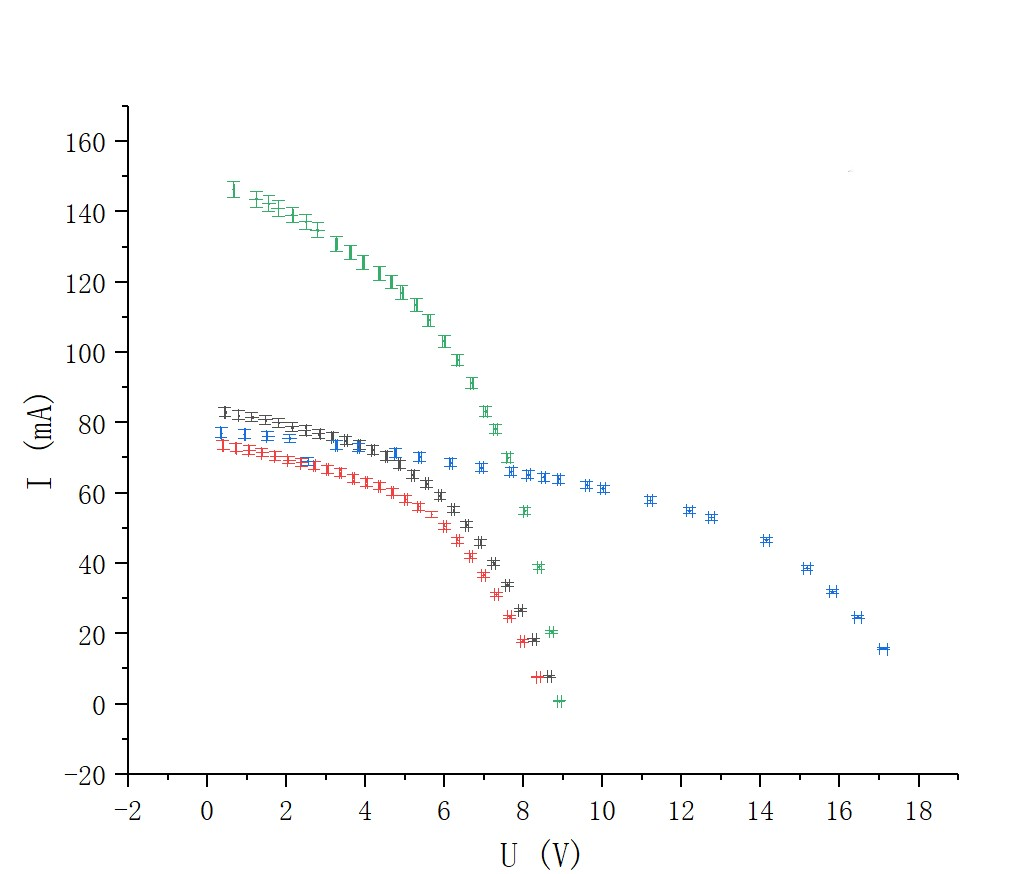
\includegraphics[scale=0.4]{P4.jpg}
\caption{Relation of $I$ and $V$}
\end{figure}
\begin{figure}[H]
\centering
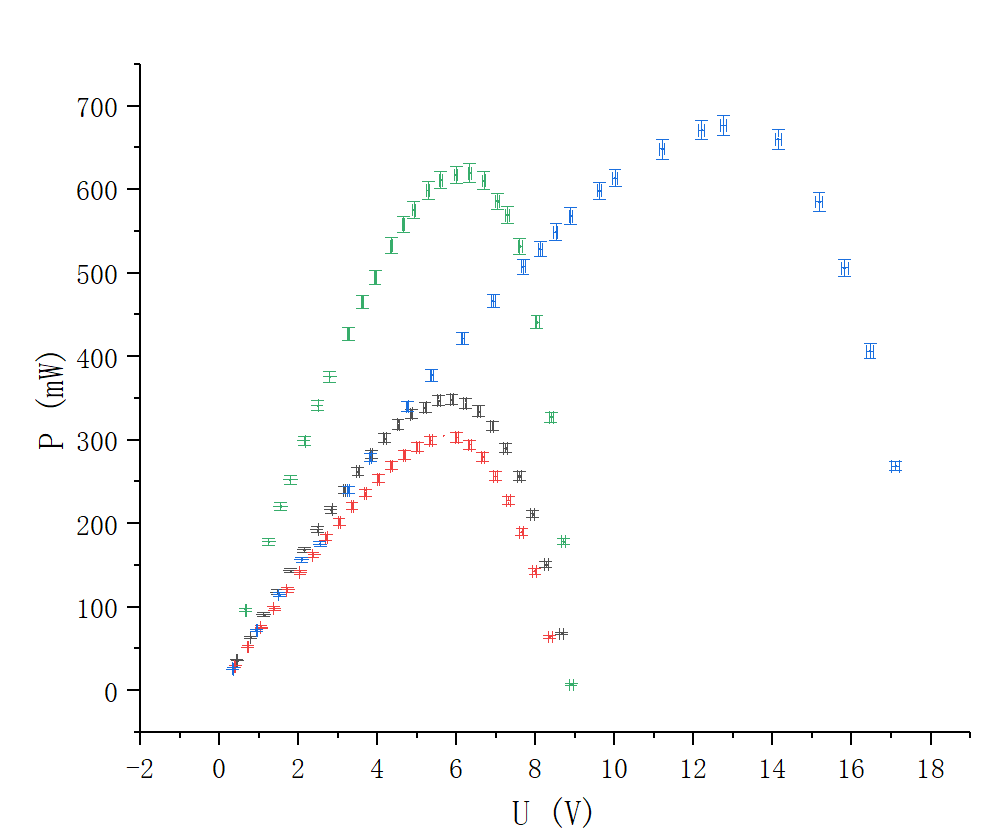
\includegraphics[scale=0.3]{P5.jpg}
\caption{Relation of $P$ and $V$}
\end{figure}
\begin{figure}[H]
\centering
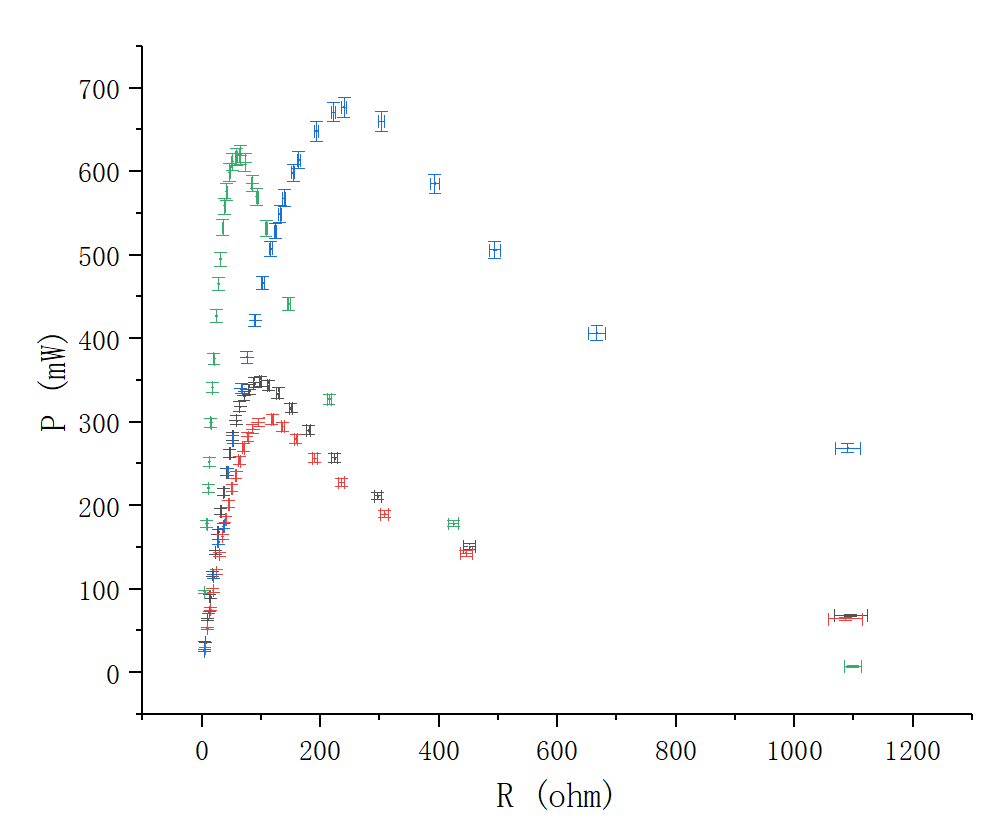
\includegraphics[scale=0.45]{P6.jpg}
\caption{Relation of $P$ and $R$}
\end{figure}
\section{Uncertainty Analysis}
\subsection{Uncertainty of Area}
$$u_A=\sqrt{(\frac{\partial A}{\partial d}\cdot u_d)^2+(\frac{\partial A}{\partial l}\cdot u_l)^2}=\sqrt{(20.9\cdot0.1)^2+(26.2\cdot0.1)^2}=3.35[cm^2]=3.35\cdot10^{-4}[m^2]$$
\subsection{Uncertainty of Solar Power per Area}
$$s_{\bar{X}}=\frac{s_X}{\sqrt{n-1}}=\frac{21.3}{2}=10.65[W/m^2]$$
$$\bigtriangleup_A=s_{\bar{X}}\cdot\frac{t_{0.95}}{\sqrt{5}}=10.65\cdot1.204=12.82[W/m^2]$$
$$\bigtriangleup_B=10[W/m^2]$$
$$u_{100}=\sqrt{\bigtriangleup_A^2+\bigtriangleup_B^2}=\sqrt{10^2+12.82^2}=16.26[W/m^2]$$
$$u_r=\frac{u_{100}}{P_{100}}\cdot100\%=\frac{16.26}{250}\cdot100\%=6.50\%$$
Similarly, $u_{120}=13.2[W/m^2],u_r=6.32\%$
\subsection{Uncertainty of Solar Power}
When the distance is 100$[cm]$,
$$u_P=\sqrt{(\frac{\partial P}{\partial A}\cdot u_A)^2+(\frac{\partial P}{\partial A}\cdot u_{100})^2}=\sqrt{(5.476\cdot10^{-2}\cdot16.26)^2+(250\cdot3.35\cdot10^{-4})^2}=0.89[W]$$
$$u_r=\frac{u_P}{P}\cdot100\%=\frac{0.89}{13.7}\cdot100\%=6.50\%$$
Similarly, when the distance is 120$[cm],u_P=0.73[W],u_r=3.22\%$
\subsection{Uncertainty of $U_{oc}$ and $I_{sc}$}
\begin{table}[H]
\centering
\begin{tabular}{|c|c|c|c|c|}
\hline
         & $U_{oc}$[V]&$I_{sc}$[mA] &$u_u$  &$u_I$  \\ \hline
100 cm    & 8.91  & 83.2  &1.35  &0.05  \\ \hline
120 cm    & 8.38  & 72.4  &1.19  &0.05  \\ \hline
series   & 18.06 & 77.2   &1.26  &0.10  \\ \hline
parallel & 9.01  & 146.7  &2.30  &0.06  \\ \hline
\end{tabular}
\end{table}
\subsection{Uncertainty of I and V}
For the first pair data, when the distance between the light source and the photovoltaic is 100$[cm]$
$$u_v=0.44\cdot0.5\%+0.01=0.01[V]$$
$$u_r=\frac{0.01}{0.44}\cdot100\%=2.27\%$$
$$u_I=83\cdot1.5\%+0.1=1.3[mA]$$
$$u_r=\frac{1.3}{85}\cdot100\%=1.53\%$$
\begin{table}[H]
\centering
\begin{tabular}{|c|c|c|c|c|c|c|c|c|}
\hline
   & \multicolumn{4}{c|}{100 cm} & \multicolumn{4}{c|}{120 cm} \\ \hline
   & U[V] &$u_v$[V] & I[mA]&$u_I$[mA]  & U[V]&$u_v$[V] & I[mA]&$u_I$[mA] \\ \hline
1  & 0.44  &0.01      & 83.0&1.3         & 0.39&0.01        & 73.7 &1.2        \\ \hline
2  & 0.78  &0.01      & 82.1&1.3         & 0.72&0.01        & 72.9 &1.2        \\ \hline
3  & 1.12  &0.02      & 81.6&1.3         & 1.05&0.02        & 72.2 &1.2        \\ \hline
4  & 1.46  &0.02      & 80.8&1.3         & 1.38&0.02        & 71.5 &1.2        \\ \hline
5  & 1.80  &0.02      & 80.0&1.3         & 1.71&0.02       & 70.5  &1.2       \\ \hline
6  & 2.14  &0.02      & 78.8&1.3         & 2.04&0.02       & 69.4  &1.1       \\ \hline
7  & 2.48  &0.02      & 77.8&1.3         & 2.37&0.02        & 68.6 &1.1        \\ \hline
8  & 2.82  &0.02      & 76.8&1.3         & 2.70&0.02        & 67.8 &1.1        \\ \hline
9  & 3.16  &0.03      & 76.0&1.2         & 3.03&0.03        & 66.7 &1.1       \\ \hline
10 & 3.50  &0.03      & 74.9&1.2         & 3.36&0.03        & 65.8 &1.1        \\ \hline
11 & 3.84  &0.03      & 73.7&1.2         & 3.69&0.03        & 64.2 &1.1        \\ \hline
12 & 4.18  &0.03      & 72.3&1.2         & 4.02&0.03        & 63.1 &1.1        \\ \hline
13 & 4.52  &0.03      & 70.5&1.2         & 4.35&0.03        & 61.9 &1.0        \\ \hline
14 & 4.86  &0.03      & 68.2&1.1         & 4.68&0.03        & 60.3 &1.0        \\ \hline
15 & 5.20  &0.04      & 65.2&1.1         & 5.01&0.04        & 58.2 &1.0        \\ \hline
16 & 5.54  &0.04      & 62.7&1.0         & 5.34&0.04        & 56.1 &0.9        \\ \hline
17 & 5.88  &0.04      & 59.3&1.0         & 5.67&0.04        & 53.8 &0.9        \\ \hline
18 & 6.22  &0.04      & 55.3&0.9         & 6.00&0.04        & 50.5 &0.9        \\ \hline
19 & 6.56  &0.04      & 51.0&0.9         & 6.33&0.04        & 46.5 &0.8        \\ \hline
20 & 6.90  &0.04      & 45.9&0.8         & 6.66&0.04        & 42.0 &0.7        \\ \hline
21 & 7.24  &0.05      & 40.1&0.7         & 6.99&0.05        & 36.7 &0.7        \\ \hline
22 & 7.58  &0.05      & 33.9&0.6         & 7.32&0.05       & 31.1  &0.6       \\ \hline
23 & 7.92  &0.05      & 26.7&0.5         & 7.65&0.05        & 24.8 &0.5        \\ \hline
24 & 8.26  &0.05      & 18.3&0.4         & 7.98&0.05        & 17.9 &0.4        \\ \hline
25 & 8.65  &0.05      & 7.9&0.2          & 8.36&0.05        & 7.7  &0.2        \\ \hline
\end{tabular}
\caption{Uncertainty for $I$ vs. $U$ relation (100 cm/120 cm configuration)}
\end{table}
\begin{table}[H]
\centering
\begin{tabular}{|c|c|c|c|c|c|c|c|c|}
\hline
   & \multicolumn{4}{c|}{series}      & \multicolumn{4}{c|}{parallel}      \\ \hline
& U[V] &$u_v$[V] & I[mA]&$u_I$[mA]  & U[V]&$u_v$[V] & I[mA]&$u_I$[mA] \\ \hline
1  & 0.34&0.01     & 77.2&1.3            & 0.66&0.01     & 146.2&2.3         \\ \hline
2  & 0.94&0.01     & 76.8&1.3            & 1.24&0.02     & 143.5&2.3          \\ \hline
3  & 1.51&0.02     & 76.2&1.3            & 1.55&0.02     & 142.3&2.2          \\ \hline
4  & 2.08&0.02     & 75.5&1.2            & 1.79&0.02     & 140.9&2.2           \\ \hline
5  & 2.54&0.02     & 69.0&1.1            & 2.15&0.02     & 139.1&2.2         \\ \hline
6  & 3.26&0.03     & 73.7&1.2            & 2.49&0.02     & 137.1&2.2	           \\ \hline
7  & 3.82&0.03     & 73.0&1.2           & 2.79&0.02      & 134.7&2.1           \\ \hline
8  & 4.76&0.03     & 71.4&1.2            & 3.29&0.03     & 130.9&2.1           \\ \hline
9  & 5.37&0.04     & 70.3&1.2            & 3.62&0.03     & 128.5&2.0         \\ \hline
10 & 6.15&0.04     & 68.6&1.1            & 3.94&0.03     & 125.6&2.0          \\ \hline
11 & 6.93&0.04     & 67.3&1.1            & 4.35&0.03     & 122.5&2.0           \\ \hline
12 & 7.68&0.05     & 66.1&1.1            & 4.65&0.03     & 120.1&1.9         \\ \hline
13 & 8.11&0.05     & 65.2&1.1            & 4.92&0.03     & 117.0&1.9          \\ \hline
14 & 8.51&0.05     & 64.5&1.1            & 5.28&0.04     & 113.4&1.8           \\ \hline
15 & 8.89&0.05     & 63.9&1.1            & 5.60&0.04     & 109.2&1.7         \\ \hline
16 & 9.61&0.06     & 62.3&1.0            & 5.99&0.04     & 103.1&1.6          \\ \hline
17 & 10.01&0.06    & 61.3&1.0            & 6.33&0.04     & 97.9&1.6          \\ \hline
18 & 11.20&0.07    & 57.9&1.0            & 6.69&0.04     & 91.3&1.5           \\ \hline
19 & 12.20&0.07    & 55.0&0.9            & 7.04&0.05     & 83.2&1.3           \\ \hline
20 & 12.75&0.07    & 53.1&0.9            & 7.28&0.05     & 78.2&1.3           \\ \hline
21 & 14.14&0.08    & 46.7&0.8            & 7.60&0.05     & 70.0&1.2           \\ \hline
22 & 15.17&0.09    & 38.6&0.7            & 8.03&0.05     & 54.9&0.9          \\ \hline
23 & 15.82&0.09    & 32.0&0.6            & 8.39&0.05     & 39.0&0.7            \\ \hline
24 & 16.46&0.09    & 24.7&0.5            & 8.71&0.05     & 20.5&0.4            \\ \hline
25 & 17.11&0.10    & 15.7&0.3            & 8.90&0.05     & 0.81&0.1         \\ \hline
\end{tabular}
\caption{Uncertainty data for the $I$ vs. $U$ relation (series/parallel configuration)}
\end{table}
\subsection{Uncertainty for P}
For the first pair data, when the distance between the light source and the photovoltaic is 100$[cm]$
$$u_p=\sqrt{(\frac{\partial p}{\partial I}u_I)^2+((\frac{\partial p}{\partial u}u_u)^2}=\sqrt{(0.44\cdot1.3)^2+(83\cdot0.01)^2}=1.01[mW]$$
$$u_r\frac{u_p}{p}\cdot100\%=\frac{1}{36.5}\cdot100\%=2.74\%$$
\begin{table}[H]
\centering
\begin{tabular}{|c|c|c|c|c|c|c|c|c|}
\hline
   & \multicolumn{4}{c|}{100 cm}      & \multicolumn{4}{c|}{120 cm}      \\ \hline
   & U[V]        & I[mA]  &P[mW] &$u_P$[mW]     & U[V]        & I[mA]    &P[mW]&$u_P$[mW]    \\ \hline
1  & 0.44        & 83.0   &36.5&1.01     & 0.39        & 73.7     &28.7 &0.87   \\ \hline
2  & 0.78        & 82.1   &64.0&1.30     & 0.72        & 72.9     &52.5 &1.13    \\ \hline
3  & 1.12        & 81.6   &91.4&2.19     & 1.05        & 72.2     &75.8 &1.92    \\ \hline
4  & 1.46        & 80.8   &118 &2.49     & 1.38        & 71.5     &98.7 &2.19    \\ \hline
5  & 1.80        & 80.0   &144 &2.83     & 1.71        & 70.5     &120  &2.49    \\ \hline
6  & 2.14        & 78.8   &169 &3.20     & 2.04        & 69.4     &142  &2.64    \\ \hline
7  & 2.48        & 77.8   &193 &3.58     & 2.37        & 68.6     &163  &2.95    \\ \hline
8  & 2.82        & 76.8   &217 &3.97     & 2.70        & 67.8     &183  &3.26    \\ \hline
9  & 3.16        & 76.0   &240 &4.42     & 3.03        & 66.7     &202  &3.89    \\ \hline
10 & 3.50        & 74.9   &262 &4.76     & 3.36        & 65.8     &221  &4.19    \\ \hline
11 & 3.84        & 73.7   &283 &5.11     & 3.69        & 64.2     &237  &4.49    \\ \hline
12 & 4.18        & 72.3   &302 &5.46     & 4.02        & 63.1     &254  &4.81    \\ \hline
13 & 4.52        & 70.5   &319 &5.82     & 4.35        & 61.9     &269  &4.73    \\ \hline
14 & 4.86        & 68.2   &331 &5.72     & 4.68        & 60.3     &282  &5.02    \\ \hline
15 & 5.20        & 65.2   &339 &6.28     & 5.01        & 58.2     &292  &5.52    \\ \hline
16 & 5.54        & 62.7   &347 &6.08     & 5.34        & 56.1     &300  &5.30    \\ \hline
17 & 5.88  		 &59.3    &349 &6.34     & 5.67        &53.8      &305  &5.54    \\ \hline
18 & 6.22        & 55.3   &344 &6.02     & 6.00        & 50.5     &303  &5.76    \\ \hline
19 & 6.56        & 51.0   &335 &6.24     & 6.33        & 46.5     &294  &5.39    \\ \hline
20 & 6.90        & 45.9   &317 &5.81     & 6.66        & 42.0     &280  &4.96    \\ \hline
21 & 7.24        & 40.1   &290 &5.45     & 6.99        & 36.7     &257  &5.23    \\ \hline
22 & 7.58        & 33.9   &257 &4.85     & 7.32        & 31.1     &228  &4.66    \\ \hline
23 & 7.92        & 26.7   &211 &4.17     & 7.65        & 24.8     &190  &4.02    \\ \hline
24 & 8.26        & 18.3   &151 &3.43     & 7.98        & 17.9     &143  &3.32    \\ \hline
25 & 8.65        & 7.9    &68.3&1.1      & 8.36        & 7.7      &64.4 &1.72    \\ \hline
\end{tabular}
\caption{Uncertainty for $P$ vs. $U$ relation (100 cm/120 cm configuration)}
\end{table}
\begin{table}[H]
\centering
\begin{tabular}{|c|c|c|c|c|c|c|c|c|}
\hline
   & \multicolumn{4}{c|}{series}      & \multicolumn{4}{c|}{parallel}      \\ \hline
   & U{[}V{]} & I{[}mA{]} & P{[}mW{]}&$u_P$[mW] & U{[}V{]} & I{[}mA{]} & P{[}mW{]}&$u_P$[mW] \\ \hline
1  & 0.34     & 77.2      & 26.2 &0.89    & 0.66     & 146.2     & 96.5  &2.11   \\ \hline
2  & 0.94     & 76.8      & 72.2 &1.44    & 1.24     & 143.5     & 178   &4.05   \\ \hline
3  & 1.51     & 76.2      & 115  &2.48    & 1.55     & 142.3     & 221   &4.44   \\ \hline
4  & 2.08     & 75.5      & 157  &2.92    & 1.79     & 140.9     & 252   &4.84   \\ \hline
5  & 2.54     & 69.0      & 175  &3.12    & 2.15     & 139.1     & 298.9 &5.49   \\ \hline
6  & 3.26     & 73.7      & 240  &4.49    & 2.49     & 137.1     & 341   &6.13   \\ \hline
7  & 3.82     & 73.0      & 279  &5.08    & 2.79     & 134.7     & 376   &6.45   \\ \hline
8  & 4.76     & 71.4      & 340  &6.10    & 3.29     & 130.9     & 431   &7.89   \\ \hline
9  & 5.37     & 70.3      & 378  &7.03    & 3.62     & 128.5     & 465.2 &8.20   \\ \hline
10 & 6.15     & 68.6      & 422  &7.30    & 3.94     & 125.6     & 495   &8.73   \\ \hline
11 & 6.93     & 67.3      & 466  &8.08    & 4.35     & 122.5     & 533   &9.44   \\ \hline
12 & 7.68     & 66.1      & 508  &9.07    & 4.65     & 120.1     & 558   &9.54   \\ \hline
13 & 8.11     & 65.2      & 528  &9.50    & 4.92     & 117.0     & 576   &9.98   \\ \hline
14 & 8.51     & 64.5      & 549  &9.90    & 5.28     & 113.4     & 599   &10.5   \\ \hline
15 & 8.89     & 63.9      & 568  &10.3    & 5.60     & 109.2     & 612   &10.5   \\ \hline
16 & 9.61     & 62.3      & 599  &10.3    & 5.99     & 103.1     & 618   &10.4   \\ \hline
17 & 10.01    & 61.3      & 614  &10.7    & 6.33     & 97.9      & 620   &10.9   \\ \hline
18 & 11.20    & 57.9      & 648  &11.9    & 6.69     & 91.3      & 611   &10.7   \\ \hline
19 & 12.20    & 55.0      & 671  &11.6    & 7.04     & 83.2      & 586   &10.1   \\ \hline
20 & 12.75    & 53.1      & 677  &12.1    & 7.28     & 78.2      & 570   &10.2   \\ \hline
21 & 14.14    & 46.7      & 660  &11.9    & 7.60     & 70.0      & 532   &9.77   \\ \hline
22 & 15.17    & 38.6      & 586  &11.2    & 8.03     & 54.9      & 441   &7.73   \\ \hline
23 & 15.82    & 32.0      & 506  &9.92    & 8.39     & 39.0      & 327   &6.19   \\ \hline
24 & 16.46    & 24.7      & 407  &8.52    & 8.71     & 20.5      & 179   &3.63   \\ \hline
25 & 17.11    & 15.7      & 269  &5.37    & 8.90     & 0.81      & 7.21  &0.89   \\ \hline
\end{tabular}
\caption{Uncertainty data for the $P$ vs. $U$ relation (series/parallel configuration)}
\end{table}
\subsection{Uncertainty of R}
For the first pair data, when the distance between the light source and the photovoltaic is 100$[cm]$
$$u_R=\sqrt{(\frac{\partial R}{\partial I}u_I)^2+((\frac{\partial p}{\partial u}u_u)^2}=\sqrt{(\frac{0.44}{83^2}\cdot1.3)^2+(\frac{0.01}{83})^2}\cdot1000=0.15[\Omega]$$
$$u_r\frac{u_R}{R}\cdot100\%=\frac{0.15}{5.3}\cdot100\%=2.76\%$$
\begin{table}[H]
\centering
\begin{tabular}{|c|c|c|c|c|c|c|c|c|}
\hline
   & \multicolumn{4}{c|}{100 cm}      & \multicolumn{4}{c|}{120 cm}      \\ \hline
   & R[$\Omega$]     &$u_R [\Omega]$  &P[mW] &$u_P$[mW]     & R[$\Omega$]     & $u_R [\Omega]$     &P[mW]&$u_P$[mW]    \\ \hline 
1  & 5.3         & 0.15   &36.5&1.01     & 5.3         & 0.16     &28.7 &0.87   \\ \hline
2  & 9.5         & 0.19   &64.0&1.30     & 9.88        & 0.21     &52.5 &1.13    \\ \hline
3  & 13.7        & 0.33   &91.4&2.19     & 14.5        & 0.37     &75.8 &1.92    \\ \hline
4  & 18.1        & 0.38   &118 &2.49     & 19.3        & 0.43     &98.7 &2.19    \\ \hline
5  & 22.5        & 0.44   &144 &2.83     & 24.3        & 0.50     &120  &2.49    \\ \hline
6  & 27.2        & 0.51   &169 &3.20     & 29.4        & 0.63     &142  &2.64    \\ \hline
7  & 31.9        & 0.59   &193 &3.58     & 34.5        & 0.71     &163  &2.95    \\ \hline
8  & 36.7        & 0.67   &217 &3.97     & 39.8        & 0.87     &183  &3.26    \\ \hline
9  & 41.6        & 0.77   &240 &4.42     & 45.4        & 0.97     &202  &3.89    \\ \hline
10 & 46.7        & 0.85   &262 &4.76     & 51.1        & 1.09     &221  &4.19    \\ \hline
11 & 52.1        & 0.94   &283 &5.11     & 57.5        & 1.21     &237  &4.49    \\ \hline
12 & 57.8        & 1.05   &302 &5.46     & 63.7        & 1.23     &254  &4.81    \\ \hline
13 & 64.1        & 1.17   &319 &5.82     & 70.3        & 1.38     &269  &4.73    \\ \hline
14 & 71.3        & 1.23   &331 &5.72     & 77.6        & 1.63     &282  &5.02    \\ \hline
15 & 79.8        & 1.48   &339 &6.28     & 86.1        & 1.69     &292  &5.52    \\ \hline
16 & 88.4        & 1.55   &347 &6.08     & 95.2        & 1.69     &300  &5.30    \\ \hline
17 & 99.2  		 & 1.80   &349 &6.34     & 105.4       & 1.91     &305  &5.54    \\ \hline
18 & 112.5       & 1.97   &344 &6.02     & 118.8       & 2.26     &303  &5.76    \\ \hline
19 & 128.6       & 2.40   &335 &6.24     & 136.1       & 2.49     &294  &5.39    \\ \hline
20 & 150.3       & 2.76   &317 &5.81     & 158.6       & 2.81     &280  &4.96    \\ \hline
21 & 180.5       & 3.39   &290 &5.45     & 190.5       & 3.88     &257  &5.23    \\ \hline
22 & 223.6       & 4.22   &257 &4.85     & 235.4       & 4.82     &228  &4.66    \\ \hline
23 & 296.6       & 5.86   &211 &4.17     & 308.5       & 6.54     &190  &4.02    \\ \hline
24 & 451.4       & 10.2   &151 &3.43     & 445.8       & 10.3     &143  &3.32    \\ \hline
25 & 1094.9      & 28.4   &68.3&1.1      & 1085.7      & 28.9     &64.4 &1.72    \\ \hline
\end{tabular}
\caption{Uncertainty for $P$ vs. $R$ relation (100 cm/120 cm configuration)}
\end{table}
\begin{table}[H]
\centering
\begin{tabular}{|c|c|c|c|c|c|c|c|c|}
\hline
   & \multicolumn{4}{c|}{series}      & \multicolumn{4}{c|}{parallel}      \\ \hline
   & R[$\Omega$]     &$u_R [\Omega]$  &P[mW] &$u_P$[mW]     & R[$\Omega$]     & $u_R [\Omega]$     &P[mW]&$u_P$[mW]    \\ \hline 
1  & 4.40     & 0.15      & 26.2 &0.89    & 4.51     & 0.09     & 96.5  &2.11   \\ \hline
2  & 12.2     & 0.24      & 72.2 &1.44    & 8.64     & 0.20     & 178   &4.05   \\ \hline
3  & 19.8     & 0.43      & 115  &2.48    & 10.9     & 0.22     & 221   &4.44   \\ \hline
4  & 27.5     & 0.51      & 157  &2.92    & 12.7     & 0.24     & 252   &4.84   \\ \hline
5  & 36.8     & 0.65      & 175  &3.12    & 15.5     & 0.28     & 298.9 &5.49   \\ \hline
6  & 44.2     & 0.83      & 240  &4.49    & 18.2     & 0.33     & 341   &6.13   \\ \hline
7  & 52.3     & 0.95      & 279  &5.08    & 20.7     & 0.36     & 376   &6.45   \\ \hline
8  & 66.7     & 1.20      & 340  &6.10    & 24.9     & 0.46     & 431   &7.89   \\ \hline
9  & 76.4     & 1.42      & 378  &7.03    & 28.2     & 0.50     & 465.2 &8.20   \\ \hline
10 & 89.7     & 1.55      & 422  &7.30    & 31.7     & 0.55     & 495   &8.73   \\ \hline
11 & 103.0    & 1.78      & 466  &8.08    & 35.5     & 0.63     & 533   &9.44   \\ \hline
12 & 116.2    & 2.08      & 508  &9.07    & 38.7     & 0.66     & 558   &9.54   \\ \hline
13 & 124.4    & 2.23      & 528  &9.50    & 42.1     & 0.73     & 576   &9.98   \\ \hline
14 & 131.9    & 2.38      & 549  &9.90    & 46.6     & 0.82     & 599   &10.5   \\ \hline
15 & 139.1    & 2.52      & 568  &10.3    & 51.3     & 0.88     & 612   &10.5   \\ \hline
16 & 154.3    & 2.66      & 599  &10.3    & 58.1     & 0.98     & 618   &10.4   \\ \hline
17 & 163.3    & 2.84      & 614  &10.7    & 64.7     & 1.13     & 620   &10.9   \\ \hline
18 & 193.4    & 3.55      & 648  &11.9    & 73.3     & 1.28     & 611   &10.7   \\ \hline
19 & 221.8    & 3.85      & 671  &11.6    & 84.6     & 1.45     & 586   &10.1   \\ \hline
20 & 240.1    & 4.28      & 677  &12.1    & 93.1     & 1.67     & 570   &10.2   \\ \hline
21 & 302.8    & 5.46      & 660  &11.9    & 108.6    & 1.99     & 532   &9.77   \\ \hline
22 & 393.0    & 7.50      & 586  &11.2    & 146.3    & 2.56     & 441   &7.73   \\ \hline
23 & 494.4    & 9.69      & 506  &9.92    & 215.1    & 4.06     & 327   &6.19   \\ \hline
24 & 666.4    & 14.0      & 407  &8.52    & 424.9    & 8.64     & 179   &3.63   \\ \hline
25 & 1089.8   & 21.8      & 269  &5.37    & 1098.6   & 14.9     & 7.21  &0.89   \\ \hline
\end{tabular}
\caption{Uncertainty data for the $P$ vs. $R$ relation (series/parallel configuration)}
\end{table}
\subsection{Uncertainty of $FF$ and $\eta$}
when the distance between the light source and the photovoltaic is 100 [cm]
$$u_{FF}=\sqrt{(\frac{\partial FF}{\partial P_m})^2+(\frac{\partial FF}{\partial V_{oc}})^2+(\frac{\partial FF}{\partial I_{sc}})^2}=\sqrt{(\frac{349\cdot1.35}{83.2^2\cdot8.91})^2+(\frac{349\cdot0.05}{83.2\cdot8.91^2})^2+(\frac{6.34}{83.2\cdot8.91})^2}=0.01$$
$$U_r=\frac{u_{FF}}{FF}\cdot100\%=\frac{0.01}{0.47}\cdot100\%=2.51\%$$
$$u_\eta=\sqrt{(\frac{\partial\eta}{\partial P_m})^2+(\frac{\partial\eta}{\partial P_{in}})^2}=\sqrt{(\frac{0.00634}{13.7})^2+(\frac{0.349\cdot0.89}{13.7^2})^2}=0.17\%$$
$$u_r=\frac{u_\eta}{\eta}\cdot100\%=\frac{0.17}{2.55}\cdot100\%=6.75\%$$
\begin{table}[H]
\centering
\begin{tabular}{|c|c|c|c|c|c|c|}
\hline
         & $FF$     & $u_{FF}$     & $u_r$      &  $\eta\%$    &  $u_{\eta}$    & $u_r$ \\ \hline
100 cm   & 0.47 & 0.01 & 2.51  & 2.55 & 0.17 &0.07  \\ \hline
120 cm   & 0.50 & 0.01 & 2.54  & 2.65 & 0.18 &0.07  \\ \hline
series   & 0.49 & 0.01 & 2.46  & 2.94 & 0.19 &0.07  \\ \hline
parallel & 0.47 & 0.01 & 2.43  & 2.70 & 0.18 &0.07  \\ \hline
\end{tabular}
\end{table}
\section{Conclusion}
In this exercise, I know about the working principle of solar cells and photovoltaic effect. In the lab work, I built a solar cell equivalent circuit to stimulate the solar cell. I changed the value of the resistance in the circuit and got the voltage and current through a multimeter, and got the power of the solar cell through a power meter, then I calculated and compared the power to get the filter factor $FF$ and working efficiency $\eta$. Also I draw the three plot about the $U$ vs. $I$, $U$ vs. $P$, and $R$ vs. $P$ relation under four conditions.
\begin{enumerate}
\item When the distance between the light source and the photovoltaic device is 100 cm:
\par$U_{oc}=8.91\pm1.35$[V], $I_{sc}=83.2\pm0.05$[mA], $P_m=349\pm6.34$[mW], $I_m=59.3\pm1$[mA], $V_m=5.88\pm0.04$[V], $R_m=99.2\pm1.8[\Omega],FF=0.47\pm0.01,\eta=2.55\pm0.17\%$
\item When the distance between the light source and the photovoltaic device is 120 cm:
\par$U_{oc}=8.38\pm1.19$[V], $I_{sc}=72.4\pm0.05$[mA], $P_m=305\pm5.54$[mW], $I_m=53.8\pm0.9$[mA], $V_m=5.67\pm0.04$[V], $R_m=105.4\pm1.91[\Omega],FF=0.450\pm0.01,\eta=2.65\pm0.18\%$
\item When the distance is 120 cm and the two devices are connected in series:
\par$U_{oc}=18.06\pm1.26$[V], $I_{sc}=77.2\pm0.1$[mA], $P_m=677\pm12.1$[mW], $I_m=53.1\pm0.9$[mA], $V_m=12.75\pm0.07$[V], $R_m=240.1\pm12.1[\Omega],FF=0.49\pm0.01,\eta=2.94\pm0.19\%$
\item When the distance is 120 cm and the two devices are connected in parallel:
\par$U_{oc}=9.01\pm2.3$[V], $I_{sc}=146.7\pm0.06$[mA], $P_m=620\pm10.9$[mW], $I_m=97.9\pm1.6$[mA], $V_m=6.33\pm0.04$[V], $R_m=64.7\pm1.13[\Omega],FF=0.47\pm0.01,\eta=2.70\pm0.18\%$
\end{enumerate}
\par For a solar cell equivalent circuit, $I$ becomes smaller as $U$ grows bigger while $P$ will increase first and then drop down. Also, $P$ will increase first and then drop down as $R$ increases.
\par In the three plot, the red dots are always at the bottom and the blacks dots are just above the red ones, which means when the distance is 120 cm, $I$ and $P$ are both at lost but when the distance is 100 cm, it has the lost $\eta$, while when the two devices are connected in series, it has the biggest $\eta$, leading to the most efficiency way of solar cell.
\section{Error Analysis}
\begin{enumerate}
\item The relative uncertainty of the solar power per area is very high, which is about $6.5\%$, I think it's because the distribution of the light on photovoltaic is not uniform enough. Additionally, the angle of the photovoltaic between the light source will also have significant effect on the solar power.
\item There is a slight difference between $I_{sc}$ and the the current when the resistance is 0. I think it's because there is still some internal resistance of the resistor which you can set to 0. Also, the wire and the photovoltaic device have their own resistances, which can explain the $R$ calculated in my table is bigger than 1000$\omega$ sometimes.
\item When the two photovoltaic devices are in parallel, I calculated the last $R$ is more than 10000$\Omega$, I examined the data and found the current is to smaller as 0.81. I thought I might make a mistake in reading the number from the multimeter. The error bar for it is more than 1000, so I eliminate the dot from the plot.
\item In the 5th,6th and 7th pair of data collected when the two devices are connected in series, the current is smaller when the voltage is bigger, which is contradict to the rule in other data. I remember when I was doing these measurement, the multimeter suddenly turned off itself. After I opened, the current is much smaller. I thought there must be some wrong with the multimeter.
\end{enumerate} 
\section{Data Sheet}
Data sheet is attach to the report
\section{Reference}
\par Applied Photovoltaics, S.R. Wenham et al. (Earthscan, 2007)
\par Krzyzosiak,M. Lab Manual of Exercise 3.
\par Qin Tian, Zeng Ming, Zhao Xijian, Krzyzosiak,M. Handbook-Uncertainty Analysis.
\end{document}